%\documentclass[12pt]{scrreprt}
\documentclass[12pt]{report} 

% language may be romanian or english (default is english)
% type may be bachelor or master (default is bachelor)
\usepackage[language=romanian, type=bachelor]{style}

\usepackage{fancyhdr}
\pagestyle{fancy}
\lhead{}
\chead{}
\renewcommand{\headrulewidth}{0.2pt}
\renewcommand{\footrulewidth}{0.2pt}

\begin{document}

\specialization{Informatică}	
\title{Design and Implementation of an AI-Based Mobile Application for Automatic Gym Exercise Posture Analysis and Feedback}					   
\author{Strugari Cristian-Silviu}											
\supervisor{Dr. Molnar Arthur}				
				
\maketitle

\newpage
\thispagestyle{empty}
\mbox{}
\newpage
\pagenumbering{roman} 

\cleardoublepage
ABSTRACT
\vspace{0.5cm}	
\hrule
\vspace{0.5cm}	

This thesis presents the design and implementation of PoseFix, an AI-based mobile application for automatic gym exercise posture analysis and feedback. Chapter 1 introduces the problem of incorrect exercise execution among amateur athletes, motivates the need for an automated solution, and outlines the structure of the work. Chapter 2 provides the theoretical background, covering pose estimation techniques, the MediaPipe BlazePose model, and a review of related work. Chapter 3 describes the system architecture, including the three-tier design comprising a Flutter mobile application, a Java Spring Boot backend, and a Python machine learning service, as well as the user journey and database design. Chapter 4 presents the implementation details of each system component. Chapter 5 covers testing and performance evaluation. Chapter 6 draws conclusions and outlines directions for future work. The primary contribution of this thesis is a working end-to-end system capable of analysing a recorded gym exercise video and returning a structured posture score, detected mistakes, and joint angle measurements.

\tableofcontents

\newpage
\pagenumbering{arabic}

\chapter{Introduction}
\label{intro}

\section{Problem Context}
\label{sec:problem}

The incorrect execution of a gym exercise is one of the main causes of injuries in amateur athletes. Most individuals train without professional supervision, leading to improper posture, insufficient range of motion, or joint misalignment. While personal trainers provide real-time correction, their services are not always accessible or affordable. Therefore, there is a growing need for intelligent systems capable of automatically analysing exercise postures and providing corrective feedback \cite{Shim2025} \cite{Sim2024}.

Common errors observed in resistance training include excessive forward lean of the torso, asymmetrical movement of the limbs, and insufficient range of motion through the targeted joints. These deviations are frequently invisible to the athlete without external observation and tend to accumulate into chronic injury over time. Studies indicate that the shoulder, lower back, and knee are the most frequently affected anatomical regions in gym-related injuries, with improper technique being a primary contributing factor \cite{Shim2025}. 

The demand for scalable, cost-effective alternatives to personal training has grown alongside the popularisation of mobile technology and computer vision. Pose estimation models now operate in real time on consumer hardware, opening the possibility of providing instant biomechanical feedback through a smartphone application.

\section{Proposed Solution}
\label{sec:solution}

This thesis proposes the design and implementation of an AI-based mobile application capable of analysing gym exercises using pose estimation techniques. The system allows users to upload a recording of themselves performing an exercise, after which computer vision algorithms extract the body key points and compute joint angles. Based on predefined rules and posture evaluation logic, the application detects common mistakes and provides structured feedback for improvement.

The proposed system, named \textbf{PoseFix}, aims to simulate the core corrective function of a personal trainer in an accessible and affordable digital format. By processing a video recording rather than requiring live streaming, the system accommodates real-world network constraints and allows users to record exercises at their own pace and in any gym environment.

\section{Technical Approach}
\label{sec:approach}

The application is developed using a Flutter-based mobile interface, a Java backend for business logic and data management, and a separate Python-based machine learning service responsible for posture analysis. Pose estimation models such as MediaPipe BlazePose \cite{Tetreault2016} or similar lightweight neural networks are integrated into the ML service to detect body landmarks from video frames. The system stores only relevant metadata in a Supabase database, while video data is processed temporarily and discarded after the analysis. The implementation includes requirement specification, system architecture design, algorithmic posture evaluation, testing, and performance validation.

\section{Structure of the Thesis}
\label{sec:structure}

The remainder of this thesis is organised as follows. Chapter 2 provides the theoretical background on pose estimation, the MediaPipe BlazePose model, and related work in automated exercise coaching. Chapter 3 describes the overall system architecture, the user journey, and the database design. Chapter 4 presents the implementation of each system component in detail. Chapter 5 covers testing methodology and performance results. Chapter 6 draws conclusions and identifies future development directions.

\section{Declaration of Generative AI and AI-Assisted Technologies in the Writing Process}
\label{sec:ai-declaration}

During the preparation of this work the author used Claude (Anthropic) in order to assist with phrasing, structural suggestions, and code review during the development phase. After using this tool, the author reviewed and edited the content as needed and takes full responsibility for the content of the thesis.


\chapter{Theoretical Background}
\label{chap:theory}

This chapter presents the theoretical foundations underlying the PoseFix system. It begins with an overview of pose estimation as a computer vision discipline, followed by a detailed description of the MediaPipe BlazePose model used in this work. The chapter concludes with a review of related work in the field of automated exercise analysis.

\section{Pose Estimation in Computer Vision}
\label{sec:pose-estimation}

Pose estimation is the computer vision task of detecting and localising the key anatomical landmarks of the human body — typically joints such as shoulders, elbows, wrists, hips, knees, and ankles — from image or video input. The output is commonly represented as a set of coordinates, called a skeleton or pose graph, describing the spatial position of each landmark.

\subsection{2D vs. 3D Pose Estimation}
\label{subsec:2d-3d}

Early approaches to pose estimation operated exclusively in two dimensions, producing $(x, y)$ coordinates for each landmark within the image plane. Two-dimensional methods are computationally inexpensive and sufficient for many tasks, but they suffer from a fundamental limitation: depth ambiguity. Because the image is a projection of three-dimensional space onto a flat sensor, two different three-dimensional configurations can produce identical two-dimensional observations. This is particularly problematic in exercise analysis, where subtle out-of-plane deviations — such as a slight lean of the torso — may be invisible in the image plane.

Modern models, including MediaPipe BlazePose, estimate a third coordinate $z$, approximating the depth of each landmark relative to the centre of the body. While this estimate is less accurate than dedicated depth-camera measurements, it provides sufficient information to detect gross postural errors such as excessive back lean and arm asymmetry. In this work, three-dimensional angle computation is used for all critical joint evaluations, as described in Chapter 4.

\subsection{Detection Approaches}
\label{subsec:detection-approaches}

Pose estimation methods broadly fall into two categories: top-down and bottom-up. Top-down approaches first detect a bounding box around each person in the image and then apply a separate pose estimation model within each box. This produces high accuracy when individuals are well separated but is sensitive to missed detections. Bottom-up approaches detect all landmarks in the image simultaneously and then associate them into individual skeletons. Bottom-up methods scale better to crowded scenes but may produce lower per-person accuracy.

MediaPipe BlazePose uses a top-down pipeline optimised for single-person video, which is the relevant scenario for self-recorded gym exercise videos. A lightweight detector locates the person in the first frame, and a tracking model maintains the skeleton estimate across subsequent frames without re-running full detection on every frame. This design enables real-time performance on mobile hardware.

\section{MediaPipe BlazePose}
\label{sec:blazepose}

MediaPipe BlazePose is an open-source pose estimation model developed by Google and released as part of the MediaPipe framework. It produces 33 three-dimensional landmarks covering the full body, including the face, torso, arms, and legs. Each landmark is annotated with a visibility score indicating the model's confidence that the point is visible and unoccluded in the frame.

\begin{figure}[htbp]
    \centering
    \includegraphics[width=0.55\textwidth]{./figures/blazepose_landmarks.png}
    \caption{The 33 body landmarks produced by MediaPipe BlazePose, covering the full body skeleton.}
    \label{fig:blazepose}
\end{figure}

\subsection{Architecture}
\label{subsec:blazepose-arch}

BlazePose consists of two neural network stages. The first stage is a lightweight person detector based on a single-shot detection architecture, responsible for localising the subject and providing a region of interest. The second stage is a regression network that maps the cropped image region to the 33 landmark coordinates and their visibility scores. The regression approach — predicting coordinates directly rather than generating heatmaps — enables sub-pixel accuracy and low latency.

In video mode, which is the mode used in this project, the framework skips the person detector on all frames after the first by using the previous frame's landmark positions to estimate the region of interest for the current frame. This tracking-based approach significantly reduces computational load and enables smooth landmark trajectories, which is important for reliable angle calculations over time.

\subsection{Coordinate System and Landmark Indices}
\label{subsec:coordinates}

Each landmark is represented as a normalised coordinate $(x, y, z)$ where $x$ and $y$ are normalised to the image width and height respectively, and $z$ represents depth relative to the midpoint of the hips. The sign convention for $z$ places landmarks closer to the camera at more negative values. The 33 landmarks are indexed from 0 to 32, with the following indices relevant to the exercises analysed in this project:

\begin{table}[htbp]
\begin{center}
\begin{tabular}{|p{60pt}|p{60pt}|p{200pt}|}
\hline
\textbf{Index} & \textbf{Side} & \textbf{Landmark} \\
\hline
11 & Left  & Shoulder \\
\hline
12 & Right & Shoulder \\
\hline
13 & Left  & Elbow \\
\hline
14 & Right & Elbow \\
\hline
15 & Left  & Wrist \\
\hline
16 & Right & Wrist \\
\hline
23 & Left  & Hip \\
\hline
24 & Right & Hip \\
\hline
25 & Left  & Knee \\
\hline
26 & Right & Knee \\
\hline
\end{tabular}
\end{center}
\caption{BlazePose landmark indices used in the posture evaluation logic of PoseFix.}
\label{tab:landmarks}
\end{table}

\section{Joint Angle Computation}
\label{sec:angles}

A joint angle is defined as the angle at vertex point $B$ formed by the vectors $\overrightarrow{BA}$ and $\overrightarrow{BC}$, where $A$, $B$, and $C$ are three landmark coordinates. In three-dimensional space, this is computed using the dot product formula:

\begin{equation}
    \theta = \arccos \left( \frac{\overrightarrow{BA} \cdot \overrightarrow{BC}}{\left\|\overrightarrow{BA}\right\| \cdot \left\|\overrightarrow{BC}\right\|} \right)
    \label{eq:angle3d}
\end{equation}

The result $\theta$ is expressed in degrees and represents the opening angle at the joint. For example, the back angle is computed with the left shoulder as point $A$, the left hip as vertex $B$, and the left knee as point $C$. A value near 180° indicates an upright posture, while a value significantly below 90° indicates excessive forward or backward lean.

Numerical stability is ensured by clipping the cosine value to the range $[-1, 1]$ before applying $\arccos$, preventing domain errors due to floating-point rounding.

\section{Related Work}
\label{sec:related}

The use of computer vision for exercise analysis has attracted growing research interest in parallel with the improvement of real-time pose estimation models.

Sim et al. \cite{Sim2024} proposed a virtual gym assistant using MediaPipe for pose estimation, demonstrating the feasibility of rule-based posture evaluation using landmark coordinates. Their system detected incorrect squat and bicep curl form using angle thresholds applied to 2D landmarks. The present work extends this approach to 3D coordinates and introduces a proportional scoring model rather than binary pass/fail judgements.

Tetreault \cite{Tetreault2016} studied behavioural interventions for reducing unsafe weight-lifting techniques in a gym environment. While that work focused on behavioural coaching rather than computer vision, it established a quantitative taxonomy of common form errors in resistance training that informs the rule design in this project.

Shim et al. \cite{Shim2025} provide a contemporary review of injury mechanisms in resistance training, identifying the shoulder, lumbar spine, and knee as the most commonly injured regions and attributing a significant proportion of injuries to technique errors. This motivates the specific checks implemented in the posture evaluation module, particularly the back angle and range-of-motion rules.

Compared to existing systems, PoseFix differs in three key respects: it operates on user-recorded video rather than live streaming, it uses a three-tier microservice architecture that cleanly separates UI, business logic, and ML concerns, and it returns a structured machine-readable result (score, mistake list, angle summary) rather than only a visual overlay.

\chapter{System Architecture and Design}
\label{chap:architecture}

This chapter presents the overall design of the PoseFix system. It describes the high-level three-tier architecture, the user journey from registration through posture feedback, and the relational database schema.

\section{High-Level Architecture}
\label{sec:high-level}

PoseFix is structured as a three-tier microservice system, with a clear separation of concerns between the mobile client, the backend server, and the machine learning service. Figure \ref{fig:architecture} illustrates the relationships between these components.

\begin{figure}[htbp]
    \centering
    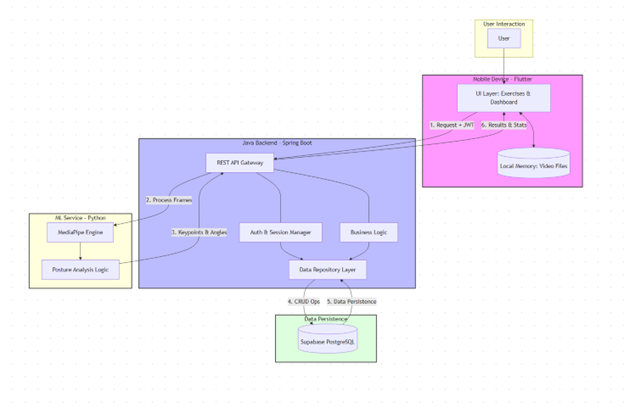
\includegraphics[width=0.85\textwidth]{./figures/system_architecture.png}
    \caption{High-level architecture of the PoseFix system, showing the three-tier structure and the data flow between components.}
    \label{fig:architecture}
\end{figure}

The \textbf{Flutter mobile application} serves as the user interface layer. It communicates exclusively with the Java backend over HTTP and relies on the Supabase client SDK only for authentication token management. The mobile client never contacts the Python ML service directly.

The \textbf{Java Spring Boot backend} is responsible for authentication enforcement, business logic, data persistence, and orchestration. When a user submits a video for analysis, the backend stores the file locally, forwards it to the Python service by reference, receives the result, persists it to the database, and returns it to the mobile client. The backend is also the sole layer that communicates with the Supabase PostgreSQL database.

The \textbf{Python FastAPI ML service} is a stateless microservice with a single responsibility: accepting a file path and an exercise identifier, processing the video using MediaPipe BlazePose, evaluating the pose against rule-based heuristics, and returning a structured JSON result. It holds no database connection and no user state.

\textbf{Supabase} provides two infrastructure services: the authentication layer, where user identity is managed and JWT tokens are issued, and the PostgreSQL database, where all application data is persisted.

This architecture offers several advantages relevant to the thesis context. The ML service can be developed, tested, and restarted independently of the backend. The backend can be extended with new business features without modifying the ML logic. The mobile client requires only knowledge of the backend API contract.

\subsection{Technology Stack}
\label{subsec:tech-stack}

\begin{table}[htbp]
\begin{center}
\begin{tabular}{|p{100pt}|p{200pt}|}
\hline
\textbf{Layer} & \textbf{Technology} \\
\hline
Mobile & Flutter (Dart), Supabase Auth SDK, GoRouter, Provider \\
\hline
Backend & Java 17, Spring Boot 3.x, Spring Security, Spring Data JPA \\
\hline
ML Service & Python 3.11, FastAPI, MediaPipe Tasks API, OpenCV, NumPy \\
\hline
Database & Supabase (PostgreSQL 15), Row Level Security \\
\hline
Authentication & Supabase Auth (JWT) \\
\hline
\end{tabular}
\end{center}
\caption{Technology stack used in the PoseFix system.}
\label{tab:techstack}
\end{table}

\section{User Journey}
\label{sec:user-journey}

Figure \ref{fig:userjourney} presents the complete user journey through the PoseFix application, from initial registration to viewing posture feedback and tracking progress.

\begin{figure}[htbp]
    \centering
    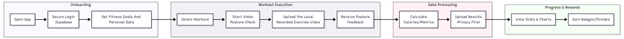
\includegraphics[width=0.90\textwidth]{./figures/user_journey.png}
    \caption{User journey through the PoseFix application, covering onboarding, workout execution, data processing, and progress tracking.}
    \label{fig:userjourney}
\end{figure}

The journey is divided into four phases.

\textbf{Onboarding} covers initial registration via Supabase Auth, followed by the user entering personal data: name, birth date, height, weight, and sex. This data is stored in the \texttt{profiles} table and used for contextualisation of feedback in future versions.

\textbf{Workout Execution} is the core operational loop. The user creates a workout session and adds one or more exercises to it, each with its own sets, reps, and load. For any exercise within the session, the user may record a video of themselves performing that exercise and upload it for analysis. The system returns a posture score, a list of detected mistakes with severity ratings, and a summary of measured joint angles specific to that exercise entry.

\textbf{Data Processing} occurs server-side and is transparent to the user. The backend receives the video, stores it temporarily, invokes the ML service, persists the result linked to the specific workout exercise entry, and deletes the video file. Only the structured analysis metadata is retained in the database.

\textbf{Progress and Tracking} allows the user to review their workout history, track weight trends over time, and compare posture scores across sessions to observe improvement.

\section{Database Design}
\label{sec:database}

The database schema consists of six tables managed by Supabase PostgreSQL. Figure \ref{fig:erd} illustrates the entity-relationship structure.

\begin{figure}[htbp]
    \centering
    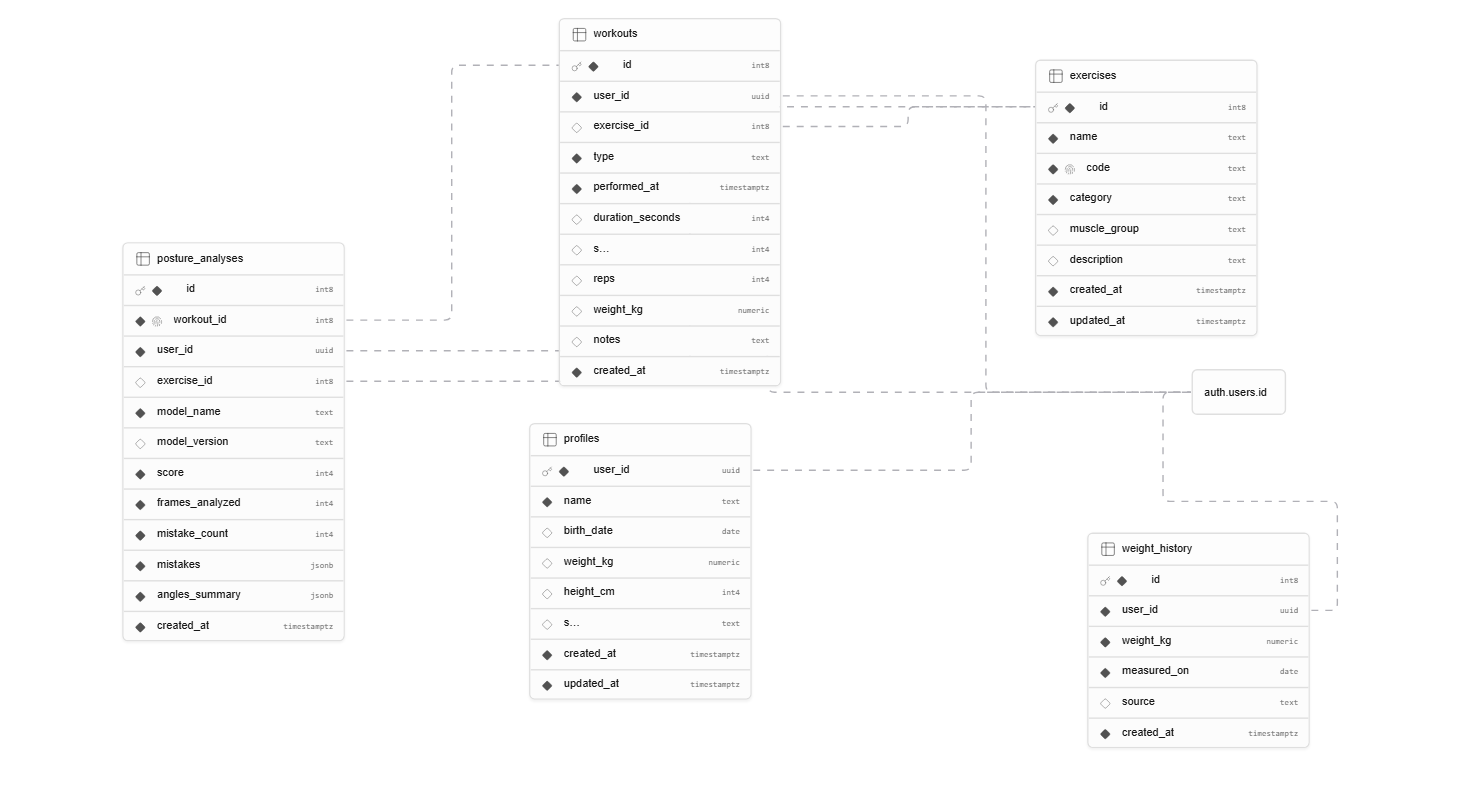
\includegraphics[width=0.85\textwidth]{./figures/erd_diagram.png}
    \caption{Entity-relationship diagram of the PoseFix database schema.}
    \label{fig:erd}
\end{figure}

\textbf{profiles} holds one record per user, linked to the Supabase \texttt{auth.users} table via the \texttt{user\_id} primary key. It stores name, birth date, height, weight, and sex. An update trigger automatically maintains the \texttt{updated\_at} timestamp.

\textbf{weight\_history} records one weight measurement per user per calendar day, enforced by a unique index on \texttt{(user\_id, measured\_on)}. This design prevents multiple daily entries that could distort trend visualisations.

\textbf{exercises} is a static reference table defining the supported exercises by name, code, category, and muscle group. The \texttt{code} column (e.g. \texttt{lat\_pulldown}) is used as a stable identifier for routing within the ML service.

\textbf{workouts} records a training session at the session level. Each row is owned by a user and stores the session timestamp, type, total duration, and optional notes. Crucially, it does not store per-exercise details such as sets, reps, or load — these are delegated to the \texttt{workout\_exercises} table, allowing a single session to contain multiple exercises.

\textbf{workout\_exercises} is a line-item table that links a workout session to a specific exercise and captures the execution parameters: \texttt{sets}, \texttt{reps}, \texttt{weight\_kg}, and \texttt{order\_index}. The \texttt{order\_index} field preserves the sequence in which exercises were performed within the session. This design normalises the schema and removes the one-exercise-per-session constraint that would otherwise limit the application's utility.

\textbf{posture\_analyses} holds the result of a video analysis for a specific exercise within a workout. It is linked one-to-one with a \texttt{workout\_exercises} row via the \texttt{workout\_exercise\_id} foreign key, ensuring that each individual exercise entry can have at most one analysis. The \texttt{mistakes} and \texttt{angles\_summary} columns are stored as JSONB, allowing the flexible structure returned by the ML service to be persisted without a fixed schema. Additional metadata includes the model name and version used for the analysis, the number of frames processed, and the total mistake count.

The relationships between tables follow a clear ownership hierarchy:

\begin{equation}
    \texttt{auth.users} \xrightarrow{1:1} \texttt{profiles} \xrightarrow{1:N} \texttt{workouts} \xrightarrow{1:N} \texttt{workout\_exercises} \xrightarrow{1:1} \texttt{posture\_analyses}
    \label{eq:dbrel}
\end{equation}

The \texttt{exercises} reference table participates in the schema via a foreign key from \texttt{workout\_exercises}, and independently from \texttt{posture\_analyses}, so that the analysed exercise is always traceable regardless of whether the originating workout entry is still present. Weight history is independently owned by the user and does not participate in the workout chain.

\chapter{Application Requirements and Specification}
\label{chap:requirements}

This chapter formalises the requirements of the PoseFix application and specifies the system at the level of its external interfaces. It begins with the functional requirements organised by feature area, continues with non-functional requirements, presents the principal use cases, and concludes with the REST API specification, key interaction sequences, and the operational constraints under which the system is designed to run. The contents of this chapter reflect the application as it is implemented, not an idealised future version of it.

\section{Functional Requirements}
\label{sec:functional}

The functional scope of PoseFix is divided into five feature areas: authentication and identity, profile management, weight tracking, workout and exercise logging, and posture analysis.

\subsection{Authentication and Identity}
\label{subsec:fr-auth}

\textbf{FR-1.} The system shall allow a user to create an account using an email address and a password. Registration is performed through the Supabase authentication service.

\textbf{FR-2.} The system shall allow a registered user to sign in with email and password, receiving a JWT access token on success.

\textbf{FR-3.} The system shall allow a signed-in user to sign out, invalidating the local session.

\textbf{FR-4.} The backend shall validate every incoming JWT access token against the Supabase authentication service and reject requests whose tokens are missing, expired, or invalid on any authenticated endpoint.

\textbf{FR-5.} The backend shall expose an identity-echo endpoint that returns the authenticated user's identifier and email, used to verify that the authentication pipeline is functioning correctly.

\subsection{Profile Management}
\label{subsec:fr-profile}

\textbf{FR-6.} The system shall allow an authenticated user to retrieve their own profile, containing name, birth date, weight, height, and sex.

\textbf{FR-7.} The system shall allow an authenticated user to create or update their profile. When a profile does not yet exist, the update operation shall create it, using the authenticated user identifier.

\textbf{FR-8.} The name field shall be required and non-blank. The sex field, when provided, shall take the value \texttt{male} or \texttt{female}. Remaining fields shall be optional.

\subsection{Weight Tracking}
\label{subsec:fr-weight}

\textbf{FR-9.} The system shall allow an authenticated user to log the current day's weight. At most one weight entry per user per calendar day shall be stored; a second submission on the same day shall overwrite the first.

\textbf{FR-10.} The system shall maintain a history of the user's weight entries and return, on request, the 30 most recent entries ordered from newest to oldest.

\textbf{FR-11.} Each time a new daily weight is logged, the system shall also update the \texttt{weight\_kg} field in the user's profile so that the profile reflects the latest measurement.

\subsection{Workout and Exercise Logging}
\label{subsec:fr-workout}

\textbf{FR-12.} The system shall expose a read-only catalogue of supported exercises, each with a stable machine-readable code, a display name, a category, a muscle group, and a textual description.

\textbf{FR-13.} The system shall allow an authenticated user to create a workout session. A session records the session type (\texttt{gym}, \texttt{run}, or \texttt{swim}), the performed timestamp, an optional total duration in seconds, and optional free-text notes.

\textbf{FR-14.} A workout session shall contain zero or more exercise entries. Each entry references an exercise from the catalogue and records the number of sets, the number of repetitions, an optional load in kilograms, and an ordinal position within the session.

\textbf{FR-15.} The system shall allow an authenticated user to append an additional exercise entry to an existing workout session that they own.

\textbf{FR-16.} The system shall allow an authenticated user to list their workout sessions, ordered from most recent to least recent, and to retrieve the full details of a single session by identifier. Sessions belonging to other users shall not be accessible.

\subsection{Posture Analysis}
\label{subsec:fr-analysis}

\textbf{FR-17.} The system shall allow an authenticated user to upload a video of themselves performing a specific exercise entry within one of their workout sessions. Accepted file types are \texttt{.mp4} and \texttt{.mov}. Empty files shall be rejected.

\textbf{FR-18.} Upon receiving a video, the system shall invoke the machine learning service to perform pose estimation and rule-based posture evaluation, producing a numeric score between 0 and 100, a list of detected mistakes with severity levels, and a summary of measured joint angles.

\textbf{FR-19.} The system shall persist the result of each analysis and associate it with the specific workout exercise entry for which the video was uploaded. At most one analysis per workout exercise entry shall be stored; a second attempt shall be rejected with a conflict error.

\textbf{FR-20.} For the lat pulldown exercise, the machine learning service shall evaluate the following aspects of form: camera angle adequacy (limb visibility), back lean (through the three-dimensional shoulder–hip–knee angle), arm symmetry during the pull (through the vertical offset between elbows), and range of motion (through the normalised descent of the wrists relative to the shoulders).

\textbf{FR-21.} The system shall report back to the mobile client the score, the list of mistakes, and the angle summary in a single response.

\section{Non-Functional Requirements}
\label{sec:nonfunctional}

The non-functional requirements describe the quality attributes the system shall exhibit. They are grouped by concern.

\subsection{Security}
\label{subsec:nfr-security}

\textbf{NFR-1.} All endpoints that handle user-specific data shall require a valid JWT access token. Only the health endpoint and the exercise catalogue shall be publicly accessible.

\textbf{NFR-2.} Each database query involving user-owned data shall be scoped to the authenticated user identifier. The backend shall never return data belonging to one user in response to a request made by a different user.

\textbf{NFR-3.} The Supabase service-role key shall be held only on the backend and shall not be transmitted to or stored on any client.

\textbf{NFR-4.} All passwords shall be handled exclusively by the Supabase authentication service; the application's backend and database shall not store passwords in any form.

\subsection{Performance and Responsiveness}
\label{subsec:nfr-performance}

\textbf{NFR-5.} Non-analysis API requests (authentication echo, profile read/write, workout listing, exercise listing, weight log) shall complete within approximately 500 milliseconds under typical conditions.

\textbf{NFR-6.} A posture analysis of a short video clip (typically 5–15 seconds of lat pulldown footage) shall complete within a time budget suitable for interactive use; the machine learning service shall process frames at or near real time on consumer hardware using the MediaPipe BlazePose video mode.

\textbf{NFR-7.} The maximum accepted video file size per upload shall be 50 megabytes, enforced at the HTTP multipart layer.

\subsection{Privacy}
\label{subsec:nfr-privacy}

\textbf{NFR-8.} Videos shall be used solely as transient inputs to the analysis pipeline. Only structured analysis metadata — score, mistake list, angle summary — shall be persisted in the database.

\textbf{NFR-9.} Credentials, access tokens, and personally identifying fields shall not be written to application logs.

\subsection{Reliability}
\label{subsec:nfr-reliability}

\textbf{NFR-10.} Failure of the machine learning service shall not cause the backend to return an unhandled server error. Such failures shall be translated into a 503 \emph{Service Unavailable} response with a user-facing message.

\textbf{NFR-11.} The system shall validate inputs against declared constraints before writing to the database, and shall return structured validation error messages when constraints fail.

\textbf{NFR-12.} Database integrity shall be enforced at the schema level through foreign keys, \texttt{CHECK} constraints, and unique indexes. Application code shall not be the sole guardian of these invariants.

\subsection{Usability}
\label{subsec:nfr-usability}

\textbf{NFR-13.} The mobile application shall follow the Material 3 design system and shall remain responsive on entry-level consumer smartphones.

\textbf{NFR-14.} Error states returned by the backend shall include a machine-readable field map (for validation errors) and a human-readable message (for all errors), enabling the mobile client to surface actionable guidance to the user.

\subsection{Portability and Maintainability}
\label{subsec:nfr-portability}

\textbf{NFR-15.} The mobile client shall run on both Android and iOS from a single Flutter codebase.

\textbf{NFR-16.} The three tiers shall be independently deployable and independently upgradable. No tier shall hold in-memory state that another tier depends on beyond the scope of a single request.

\textbf{NFR-17.} The exercise evaluation logic shall be organised per exercise, so that adding support for a new exercise requires adding a new evaluator module and a routing entry in the machine learning service, without modifying the backend or the mobile client.

\section{Use Cases}
\label{sec:use-cases}

This section presents the principal use cases supported by PoseFix. The actor in every case is the \emph{Authenticated User}, except for \textbf{UC1}, where the actor is an unauthenticated visitor.

\begin{figure}[htbp]
    \centering
    \includegraphics[width=0.75\textwidth]{./figures/use_case_diagram.png}
    \caption{Use case diagram of the PoseFix application.}
    \label{fig:usecases}
\end{figure}

\subsection{UC1 --- Register and Sign In}
\label{subsec:uc1}

\textbf{Actor.} Unauthenticated visitor.\\
\textbf{Preconditions.} The user has installed the mobile application.\\
\textbf{Main flow.}
\begin{enumerate}
    \item The user opens the application and is redirected to the login screen.
    \item The user enters an email address and a password and chooses either sign-in or sign-up.
    \item The Supabase authentication service validates the credentials, creating a new account if in sign-up mode.
    \item On success, Supabase issues a JWT access token, which is retained by the mobile client.
    \item The router detects the authenticated state and redirects to the home screen.
\end{enumerate}
\textbf{Alternative flows.}
\begin{itemize}
    \item If email confirmation is required, the session is null on sign-up; the user is informed to confirm via email and returned to the login screen.
    \item If the credentials are invalid, the user is shown an error message and remains on the login screen.
\end{itemize}
\textbf{Postcondition.} The user holds a valid access token and can invoke authenticated endpoints.

\subsection{UC2 --- Manage Profile}
\label{subsec:uc2}

\textbf{Preconditions.} The user is authenticated.\\
\textbf{Main flow.}
\begin{enumerate}
    \item The user requests their profile.
    \item If no profile exists, the user enters name, birth date, height, weight, and sex, and submits.
    \item The backend validates the data, creates or updates the profile row keyed by the user identifier, and returns the saved profile.
\end{enumerate}
\textbf{Alternative flows.}
\begin{itemize}
    \item Invalid input (blank name, invalid sex) yields a 400 response with a per-field error map.
\end{itemize}
\textbf{Postcondition.} The user has a persisted profile.

\subsection{UC3 --- Log a Workout Session}
\label{subsec:uc3}

\textbf{Preconditions.} The user is authenticated; at least one exercise exists in the catalogue.\\
\textbf{Main flow.}
\begin{enumerate}
    \item The user opens the workouts screen and chooses to add a session.
    \item The user selects a session type, enters an optional duration and notes, and adds one or more exercise entries. For each entry, the user selects an exercise from the catalogue and enters sets, repetitions, and optionally a load in kilograms.
    \item The user submits the session.
    \item The backend creates the workout row and the associated exercise entries, assigning each entry a sequential ordinal position, and returns the new session identifier.
    \item The workouts screen refreshes and displays the new session at the top of the list.
\end{enumerate}
\textbf{Postcondition.} A new workout session and its exercise entries are persisted.

\subsection{UC4 --- Analyse Exercise Posture}
\label{subsec:uc4}

\textbf{Preconditions.} The user is authenticated; the target workout exercise entry exists and has not previously been analysed.\\
\textbf{Main flow.}
\begin{enumerate}
    \item The user records or selects a short video of themselves performing the exercise.
    \item The user uploads the video via the analysis endpoint, identifying the target workout exercise entry.
    \item The backend authorises the request by verifying that the workout exercise entry belongs to the authenticated user.
    \item The backend stores the video on local disk and invokes the machine learning service with the file path and the exercise identifier.
    \item The machine learning service opens the video, performs frame-by-frame pose estimation with MediaPipe BlazePose, evaluates the exercise-specific rule set, and returns a score, a list of mistakes, and an angles summary.
    \item The backend persists a posture analysis row linked to the workout exercise entry and returns the result to the mobile client.
    \item The client displays the score, the list of mistakes, and the measured angles.
\end{enumerate}
\textbf{Alternative flows.}
\begin{itemize}
    \item If the workout exercise entry does not belong to the user, the backend returns 404.
    \item If an analysis already exists for the entry, the backend returns 409.
    \item If the file is empty or of an unsupported type, the backend returns 400.
    \item If the machine learning service is unreachable, the backend returns 503.
\end{itemize}
\textbf{Postcondition.} A posture analysis row is persisted, and the client has received the structured result.

\subsection{UC5 --- Review Workout History}
\label{subsec:uc5}

\textbf{Preconditions.} The user is authenticated.\\
\textbf{Main flow.}
\begin{enumerate}
    \item The user opens the workouts screen.
    \item The client fetches the user's workout sessions, each with its embedded list of exercise entries.
    \item The user can scroll the history and, in future versions, drill into a single session to view its analyses.
\end{enumerate}
\textbf{Postcondition.} The user has viewed their workout history.

\subsection{UC6 --- Log Daily Weight}
\label{subsec:uc6}

\textbf{Preconditions.} The user is authenticated.\\
\textbf{Main flow.}
\begin{enumerate}
    \item The user submits their current weight.
    \item The backend upserts the weight entry for the current date and updates the user's profile weight field.
    \item The backend returns the stored weight entry.
\end{enumerate}
\textbf{Postcondition.} The day's weight is recorded, with the profile kept in sync.

\section{System Specification}
\label{sec:system-spec}

This section specifies the external contract of the system at the HTTP level and describes the principal cross-tier interactions.

\subsection{REST API Overview}
\label{subsec:rest-overview}

The backend exposes the endpoints listed in Table \ref{tab:endpoints}. All authenticated endpoints expect the header \texttt{Authorization: Bearer <supabase-access-token>}. Unless otherwise noted, requests and responses use JSON encoding.

\begin{table}[htbp]
\begin{center}
\begin{tabular}{|p{40pt}|p{140pt}|p{35pt}|p{150pt}|}
\hline
\textbf{Method} & \textbf{Path} & \textbf{Auth} & \textbf{Purpose} \\
\hline
GET  & \texttt{/health} & No  & Liveness probe \\
\hline
GET  & \texttt{/exercises} & No  & Exercise catalogue \\
\hline
GET  & \texttt{/me} & Yes & Echo authenticated identity \\
\hline
GET  & \texttt{/profile} & Yes & Read profile \\
\hline
PUT  & \texttt{/profile} & Yes & Create or update profile \\
\hline
GET  & \texttt{/weights} & Yes & Last 30 weight entries \\
\hline
PUT  & \texttt{/weights/today} & Yes & Upsert today's weight \\
\hline
GET  & \texttt{/workouts} & Yes & List workout sessions \\
\hline
POST & \texttt{/workouts} & Yes & Create session with exercises \\
\hline
GET  & \texttt{/workouts/\{id\}} & Yes & Session detail \\
\hline
POST & \texttt{/workouts/\{id\}/exercises} & Yes & Append exercise to session \\
\hline
POST & \texttt{/workouts/\{id\}/upload-video} & Yes & Upload video without analysis \\
\hline
POST & \texttt{/workouts/exercises/\{id\}/analyze} & Yes & Analyse video for a session exercise \\
\hline
\end{tabular}
\end{center}
\caption{REST endpoints exposed by the PoseFix backend.}
\label{tab:endpoints}
\end{table}

\subsection{Error Response Format}
\label{subsec:errors}

All error responses share a common envelope, as illustrated below. The \texttt{validationErrors} field is present only when a request body fails bean-validation constraints.

\begin{figure}[htbp]
    \centering
    \includegraphics[width=0.7\textwidth]{./figures/error_response.png}
    \caption{Shape of the error response envelope returned by the backend.}
    \label{fig:errorshape}
\end{figure}

\begin{table}[htbp]
\begin{center}
\begin{tabular}{|p{70pt}|p{280pt}|}
\hline
\textbf{Status} & \textbf{When returned} \\
\hline
400 Bad Request & Validation failure, empty upload, unsupported file type. \\
\hline
401 Unauthorized & Missing, invalid, or expired JWT. \\
\hline
404 Not Found & Resource does not belong to the authenticated user or does not exist. \\
\hline
409 Conflict & Posture analysis already exists for the target workout exercise entry. \\
\hline
503 Service Unavailable & Machine learning service cannot be reached. \\
\hline
500 Internal Server Error & Any other unhandled failure; a scrubbed message is returned to the client. \\
\hline
\end{tabular}
\end{center}
\caption{Error status codes used by the backend.}
\label{tab:errors}
\end{table}

\subsection{Posture Analysis Sequence}
\label{subsec:sequence-analysis}

Figure \ref{fig:seq-analysis} illustrates the end-to-end flow of a posture analysis request across the four components of the system. The mobile client initiates the request with a multipart upload; the backend enforces ownership, persists the video, delegates to the machine learning service, and, on return, persists the structured result before responding to the client.

\begin{figure}[htbp]
    \centering
    \includegraphics[width=0.95\textwidth]{./figures/seq_analysis.png}
    \caption{Sequence diagram of the posture analysis flow.}
    \label{fig:seq-analysis}
\end{figure}

\subsection{Authentication Sequence}
\label{subsec:sequence-auth}

Figure \ref{fig:seq-auth} illustrates the authentication flow. The mobile client obtains an access token from Supabase and attaches it to every subsequent request. The backend, through a dedicated filter, validates the token against Supabase and populates the security context before any controller is invoked.

\begin{figure}[htbp]
    \centering
    \includegraphics[width=0.9\textwidth]{./figures/seq_auth.png}
    \caption{Sequence diagram of the authentication flow.}
    \label{fig:seq-auth}
\end{figure}

\section{Constraints and Assumptions}
\label{sec:constraints}

The system is designed under a number of explicit constraints and assumptions, which shape both its architecture and its evaluation.

\textbf{Co-located filesystem.} The backend passes the absolute path of the uploaded video to the machine learning service, which reads the file directly from disk. Consequently, the two processes are assumed to share a filesystem, whether by running on the same host or by mounting a shared volume. This design reduces network overhead and simplifies the machine learning service but precludes fully independent horizontal scaling of the two tiers.

\textbf{Single-exercise scope for the machine learning service.} In its current state, the machine learning service implements posture evaluation rules only for the lat pulldown exercise (exercise identifier 1). The architecture accommodates additional exercises through a registry pattern inside the service, but the thesis scope is limited to a single exercise to allow for thorough validation.

\textbf{Supabase as the authentication provider.} User identity is outsourced entirely to Supabase. The backend does not store user credentials and does not issue its own tokens; it merely validates tokens produced by Supabase. This decision trades implementation burden for a dependency on a third-party service.

\textbf{Video as a transient input.} The system is designed on the premise that videos are not retained as first-class user content. While the current implementation leaves the uploaded video on disk for post-mortem debugging, the intended production behaviour is to delete the video immediately after analysis, consistent with the privacy requirement \textbf{NFR-8}.

\textbf{One analysis per workout exercise entry.} The schema enforces a unique analysis per workout exercise row. This simplifies the data model and avoids ambiguity about which analysis represents the user's performance for a given logged set of reps.

\textbf{Mobile-first client scope.} The client is assumed to be a mobile device in portrait orientation. A web client is technically possible from the same Flutter codebase but is not a target of the current thesis.

\textbf{Single-user session model.} Each request is assumed to originate from a single authenticated user. The architecture does not support shared or collaborative workouts.

\textbf{Network availability for analysis.} The analysis flow requires network connectivity between the mobile client, the backend, and the machine learning service. Offline analysis on the device is not supported in the current scope.


\input{chapters/chapter6_conclusions}

\bibliography{references}

\end{document}
